\documentclass{article}
\usepackage{amsfonts}
\usepackage{amssymb}
\usepackage{graphicx}
\begin{document}
\hfill Alejandro Chavez

\hfill Assignment 4 - Discrete Mathematics

\hfill \today\\

\begin{center}\begin{large}Assignment 4\end{large}\end{center}	Section 2.3 p.146
\begin{itemize}
	\item
		2) 
    \begin{itemize}
      \item
        a)
        Yes
      \item
        b)
        No
      \item
        c)
        No
    \end{itemize}
	\item
		4)
    \begin{itemize}
      \item
        a)\\
        domain: $\{x\in \mathbb{Z}; 0\le x\}$\\
        range: $\{x\in \mathbb{Z}; 0\le x \le 9\}$
      \item
        b)\\
        domain: $\{x\in \mathbb{N}\}$\\
        range: $\{x\in \mathbb{Z}; 1\le x\}$\\
      \item
        c)\\
        domain: $\{x\in \mathbb{Z}; 0\le x\}$\\
        range: $\{x\in \mathbb{Z}; 0\le x\}$\\
      \item
        d)\\
        domain: $\{x\in \mathbb{Z}; 0\le x\}$\\
        range: $\{x\in \mathbb{N}\}$\\
    \end{itemize}
	\item
		8)
    \begin{itemize}
      \item
        a) $1$
      \item
        b) $-1$
      \item
        c) $3$
      \item
        d) $1$
    \end{itemize}
	\item
		10)
      \begin{itemize}
        \item
          a) Yes
        \item
          b) No
        \item
          c) No
      \end{itemize}
	\item
		16)
      \begin{itemize}
        \item
          a) $f(x)=x+1$
        \item
          b)
        \item
          c)
        \item
          d) $f(x)=1$
      \end{itemize}
	\item
		20)\\
    $x\in \mathbb{R},0<x$\\
    Suppose $f(x)=x+1$ and $g(x)=\frac{1}{x+1}$\\
    $f(x)>x$\\
    $g(x)<\frac{1}{x}$\\
	\item
		32)\\
    $f\circ g=(x+2)^{2}+1$\\
    $g\circ f=x^{2}+3$
	\item
		46)
	\item
		58)\\
    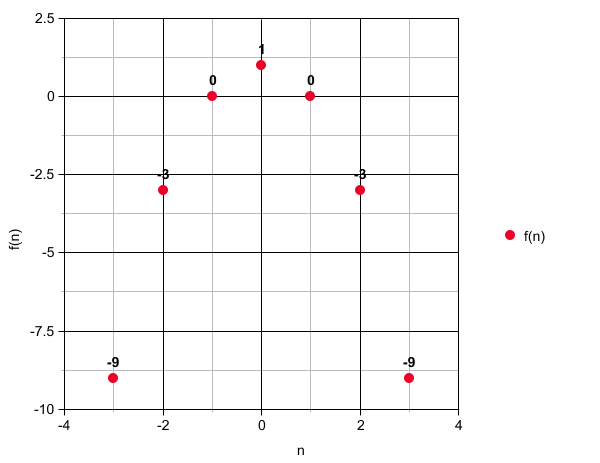
\includegraphics[scale=0.5]{graph.png}
	\item
		66)
	\item
		Lecture 9)
\end{itemize}
	Section 2.4
\begin{itemize}
	\item
		2)
    \begin{itemize}
      \item
        a) $128$
      \item
        b) $7$
      \item
        c) $2$
      \item
        d) $-256$
    \end{itemize}
	\item
		4)
    \begin{itemize}
      \item
        a) 1, -2, 3, -8
      \item
        b) 3, 3, 3, 3
      \item
        c) 8, 11, 23, 71
      \item
        d) 2, 0, 8, 0
    \end{itemize}
	\item
		8)
    \begin{itemize}
      \item
        a) $a_{n}=3+n$
      \item
        b) $a_{n}=2n+3$
      \item
        c) $a_{n}=$
    \end{itemize}
	\item
		10)
    \begin{itemize}
      \item
        a) $a_{n}=n^{2}+2$ 123, 146, 171
      \item
        b) $a_{n}=4n+3$ 47, 51, 55 
      \item
        c) $a_{n}=n+1$ 1100, 1101, 1110 
      \item
        d) 7, 7, 7
      \item
        e) $a_{n}=\frac{3^{n}+3}{3}$ 59048, 177146, 531440
      \item
        f) I have no idea
      \item
        g) 0, 0, 0
      \item
        h) $a_{0} = 2,\; a_{n} = a_{n-1}^{2}$\\
        18446744073709551616,\\ 
        340282366920938463463374607431768211456,\\
        115792089237316195423570985008687907853269984665640564039457584007913129639936
    \end{itemize}
	\item
		16)
    \begin{itemize}
      \item
        a) 10
      \item
        b) 9330
      \item
        c) 21215
      \item
        d) 511
    \end{itemize}
	\item
		19)\\
    $\sum_{j=1}^{1}=a_{1}-a_{0}$\\
    $\sum_{j=1}^{2}=a_{2}-a_{1}+a_{1}-a_{0}$\\ $\;=a_{2}-a_{0}$\\
    $\sum_{j=1}^{3}=a_{3}-a_{2}+a_{2}-a_{1}+a_{1}-a_{0}$\\ $\;=a_{3}-a_{0}$\\
    $\sum_{j=1}^{n}=a_{n}-a_{0}$
	\item
		20)
	\item
		32)
    \begin{itemize}
      \item
        a) countable\\
        $x\in \mathbb{N}$\\
        $f(x)=x+10$
      \item
        b) countable\\
        $x\in \mathbb{N}$\\
        $f(x)=-(2x-1)$
      \item
        c) not countable
      \item
        d) countable\\
        $x\in \mathbb{N}$\\
        $f(x)=10x$
    \end{itemize}
	\item
		34)
    \begin{itemize}
      \item
        a) countable\\
        $x\in \mathbb{N}$\\
        $f(x)=(6x-(-1)^{x}-3)/4$
      \item
        b) countable\\
        
      \item
        c) countable\\
        $x\in \mathbb{N}$\\
        $f(x)=|x+\frac{1}{9}| $
      \item
        d) countable 
    \end{itemize}
\end{itemize}
\end{document}
